% Full instructions available at:
% https://github.com/elauksap/focus-beamertheme

\documentclass[9pt]{beamer}
\usetheme{focus}

%%%%%%%%%%%%%%%%%%%%%%%%%%%%%%%%%%%%%%%%%%%%%%%%%%%%%%%%%%%%%%%%%%%%%
% Typography, change document font
\usepackage[tt=false, type1=true]{libertine}
\usepackage[varqu]{zi4}
\usepackage[libertine]{newtxmath}
\usepackage[T1]{fontenc}

\usepackage[protrusion=true,expansion=true]{microtype}

% Disable paragraph indentation, and increase gap
\usepackage{parskip}

%Matrix
\usepackage{tabstackengine}
\setstackEOL{;}% row separator
\setstackTAB{,}% column separator
\setstacktabbedgap{1ex}% inter-column gap 
\setstackgap{L}{1.0\normalbaselineskip}% inter-row baselineskip
\let\mat\bracketMatrixstack

\newcommand{\pth}{Figure/}
\newcommand{\ve}[1]{\mathbf{#1}}

% Copyright (C) 2018-2019 Pasquale Claudio Africa and the LaTeX community.
% A full list of contributors can be found at
%
%     https://github.com/elauksap/focus-beamertheme
% 
% This file is part of beamerthemefocus.
% 
% beamerthemefocus is free software: you can redistribute it and/or modify
% it under the terms of the GNU General Public License as published by
% the Free Software Foundation, either version 3 of the License, or
% (at your option) any later version.
% 
% beamerthemefocus is distributed in the hope that it will be useful,
% but WITHOUT ANY WARRANTY; without even the implied warranty of
% MERCHANTABILITY or FITNESS FOR A PARTICULAR PURPOSE. See the
% GNU General Public License for more details.
% 
% You should have received a copy of the GNU General Public License
% along with beamerthemefocus. If not, see <http://www.gnu.org/licenses/>.

\mode<presentation>


% DEFINE COLORS. ---------------------------------------------------------------
\definecolor{main}{RGB}{134, 161, 174}
\definecolor{main2}{RGB}{104, 131, 144}
\definecolor{textc}{RGB}{20, 20, 20}
\definecolor{background}{RGB}{255, 255, 255}

\definecolor{alert}{RGB}{180, 0, 0}
\definecolor{example}{RGB}{0, 110, 0}


% SET COLORS. ------------------------------------------------------------------
\setbeamercolor{normal text}{fg=textc, bg=background}
\setbeamercolor{alerted text}{fg=textc}
\setbeamercolor{example text}{fg=textc}

\setbeamercolor{titlelike}{fg=background, bg=main}
\setbeamercolor{frametitle}{parent={titlelike}}

\setbeamercolor{footline}{fg=background, bg=main2}

\setbeamercolor{block title}{bg=main!80!background, fg=background}
\setbeamercolor{block body}{bg=main!10!background, fg=textc}

\setbeamercolor{block title alerted}{bg=alert, fg=background}
\setbeamercolor{block body alerted}{bg=alert!10!background, fg=textc}

\setbeamercolor{block title example}{bg=example, fg=background}
\setbeamercolor{block body example}{bg=example!10!background, fg=textc}

\setbeamercolor{itemize item}{fg=textc}
\setbeamercolor{itemize subitem}{fg=textc}

\setbeamercolor{enumerate item}{fg=textc!70!black}
\setbeamercolor{enumerate subitem}{fg=textc!70!black}

\setbeamercolor{description item}{fg=textc!70!black}
\setbeamercolor{description subitem}{fg=textc!70!black}

\setbeamercolor{caption name}{fg=textc}

\setbeamercolor{section in toc}{fg=textc}
\setbeamercolor{subsection in toc}{fg=textc}
\setbeamercolor{section number projected}{bg=textc}
\setbeamercolor{subsection number projected}{bg=textc}

\setbeamercolor{bibliography item}{fg=main}
\setbeamercolor{bibliography entry author}{fg=main!70!black}
\setbeamercolor{bibliography entry title}{fg=main}
\setbeamercolor{bibliography entry location}{fg=main}
\setbeamercolor{bibliography entry note}{fg=main}

\mode<all>


\begin{document}
	\tableofcontents
	
\section{Scaling : \today}

	\begin{frame}{Scaling (Fox Stanton 1968)}
		\begin{itemize}
			\item Sometimes we want to keep all the variables in the same order of magnitude (suppose forces, moments. Displacements, rotations)
			\item We can simply scale  bya  simple multiplication of the individual dof with a non singular diagonal transofmratio matrix
			\item Eg we can have zero eigen values for rigid body displacements. Sometimes we can have the non zero eigen values range over six orders and some dof have larger strain energies than others.
		\end{itemize}
\texttt{}	\end{frame}

	\begin{frame}{Gerschgorin's theorem}
		\begin{itemize}
			\item This theorem states that every eigenvalue of a matrix $\ve{A}$ with enteties $a_{ij}$ lies in at leasat one of the disks centered at $a_{ii}$ and of radii $R_i$
			\begin{equation}
				R_i = \sum_{j\neq i } |a_{ij}|
			\end{equation}
			where $R_i$ is the sum of the absolute values of the non diagonal enteries in the $i$th row
			\item Let D($a_{ii},R_i$) be a closed disc centered at a with radius R. Such a disc is a Gershgorin disc. 
			\item Every eigen value of $A$ lies within at least one of the Gersgorin discs.
			\item Shift in orders can be because of the shift in the center without the raius isze also.  This happens when the condition number is affected by change in phyical properties (Like size of the problem) 
		\end{itemize}
	\end{frame}


	\begin{frame}
		% TODO: \usepackage{graphicx} required
		\begin{figure}
			\centering
			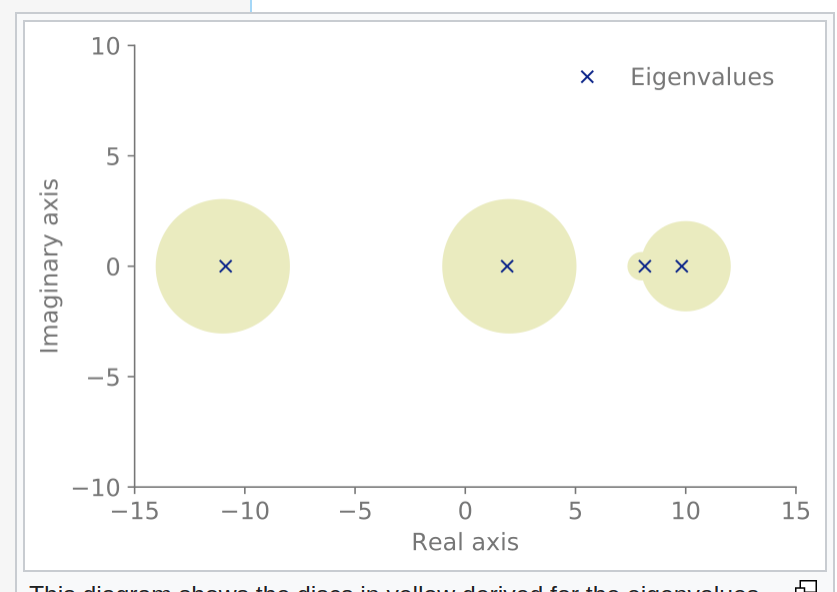
\includegraphics[width=0.7\linewidth]{Figure/screenshot001}
			\caption{}
			\label{fig:screenshot001}
		\end{figure}
		
	\end{frame}

	\begin{frame}{Scaling criteria}
		\begin{itemize}
			\item Suppose we have the potential energy in the form 
			\begin{equation}
				\Pi(X) = \frac{1}{2} X^{T}KX - X^{T}F
			\end{equation}
			\item Operated in scale coordiantes as
			\begin{equation}
				\Pi(Y) = \frac{1}{2} Y^{T}K'Y - Y^{T}F'
			\end{equation}
			where $K'=D^{T}KD \qquad F' = D^{T}F$\\
			$d_{ii}=\frac{1}{c(k_ii)^{1/2}} \qquad d_{ij}=0 \qquad i \neq j$
			\item This centers all the Gerschogorin disks at the same point namely $1/c^{2}$
			\item c =$1/n^{1/2}$ where n is the max no of nonzero elements is nonzero is a good choice.
			\item Can also be shown that they are bounded. BUT WHAT ABOUT NONLINEAR
			\item The existence of the scaling transformation requires that the diagonals > 0. Which is satisfied in positive definite matrixes.
			\item Can read Developments in structural analysis by direct energy minimization for more details.
		\end{itemize}
	\end{frame}
\end{document}